%!TEX root = main.tex

\chapter{Análisis y conclusiones}

\section{Resultados y conclusiones}
\subsection{Análisis de los resultados - velocidad del viento}
\subsubsection{Visualización de los datos}
Los gráficos \ref{fig:data_valpo_13}, \ref{fig:data_valpo_14} y \ref{fig:data_valpo_15} muestran la distribución de datos de velocidad del viento en Valparaíso a lo largo de los meses del año y las horas del día, lo cual permite visualizar la naturaleza de la intensidad del viento de forma cualitativa.
Por ejemplo, se logra apreciar que las máximas velocidades son obtenidas en los meses finales de primavera y comienzos de verano. Además, tener en cuenta que interpolación de los datos es realizada con rectas, por lo que la superficie que se expone no representa necesariamente la distribución real de los datos.\\
\begin{figure}[ht!]
     \centering
        \subfigure[Vientos Valparaíso 2013.]{
            \label{fig:data_valpo_13}
            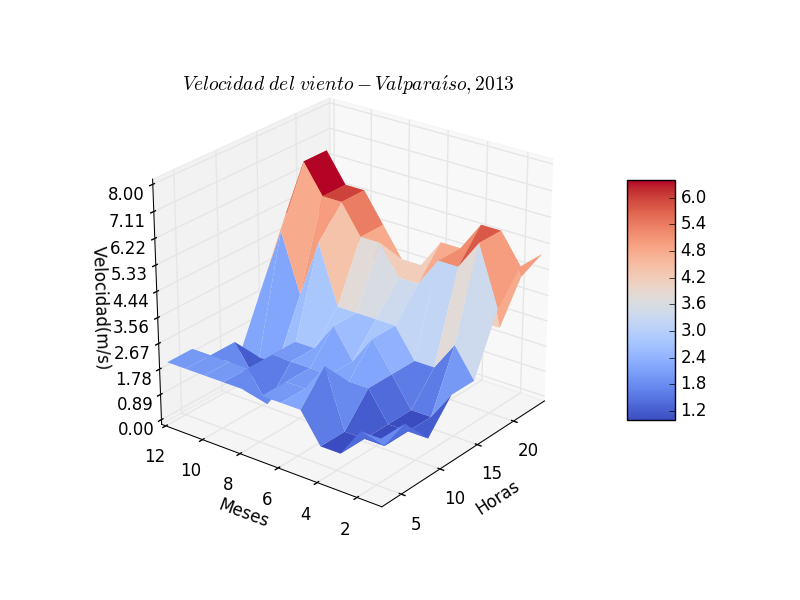
\includegraphics[width=0.4\textwidth]{figures/3d_data_2013.png}
        }%
         \subfigure[Vientos Valparaíso 2014.]{
            \label{fig:data_valpo_14}
            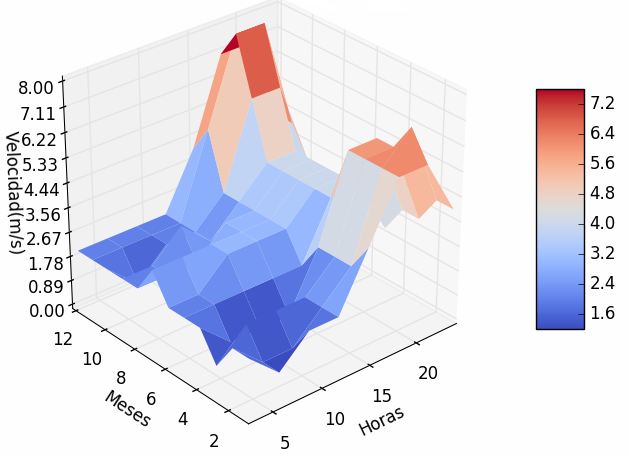
\includegraphics[width=0.4\textwidth]{figures/3d_data_2014.png}
        }\\
         \subfigure[Vientos Valparaíso 2015.]{
            \label{fig:data_valpo_15}
            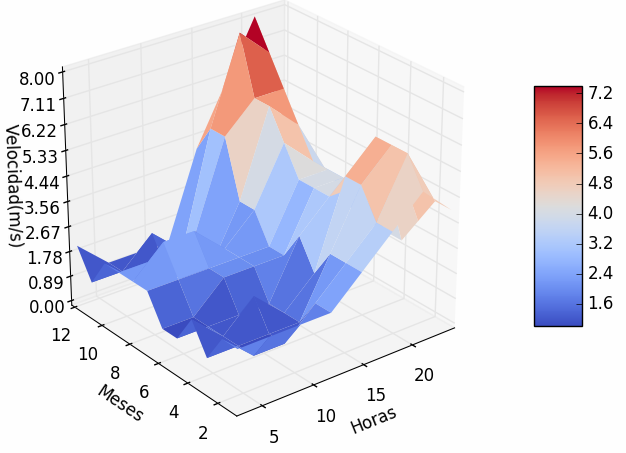
\includegraphics[width=0.4\textwidth]{figures/3d_data_2015.png}
        }%
    \caption{Superficie de datos viento de Valparaíso.\\ Fuente: Elaboración Propia.}
    \label{fig:subfigures}
\end{figure}

\subsubsection{Experimento 1, datos anuales y promedios diarios}
Las figuras \ref{fig:pso_valpo_13}, \ref{fig:pso_valpo_14} y \ref{fig:pso_valpo_15} muestran el ajuste de la distribución de Weibull a los histogramas de datos del viento (promedios diarios), con los parámetros $k$ y $c$  que se muestran en las primeras tres filas de la tabla \ref{table:stadistical_tests} determinados por el PSO. El ajuste tiene buena forma, lo cual es corroborado por los datos estadísticos obtenidos con los test previamente mencionados (RMSE, r, RB), expuestos en la tabla \ref{table:stadistical_tests}. Si se compara con la precisión conseguida en el trabajo de Carneiro et al. \cite{Carneiro15}, se aprecia que el ajuste conseguido es levemente más impreciso, sobre todo en lo relativo al test RB. Esto podría deberse a la naturaleza de los datos 
trabajados.\\
\begin{figure}[ht!]
    \centering
        \subfigure[PSO Valparaíso 2013.]{
            \label{fig:pso_valpo_13}
            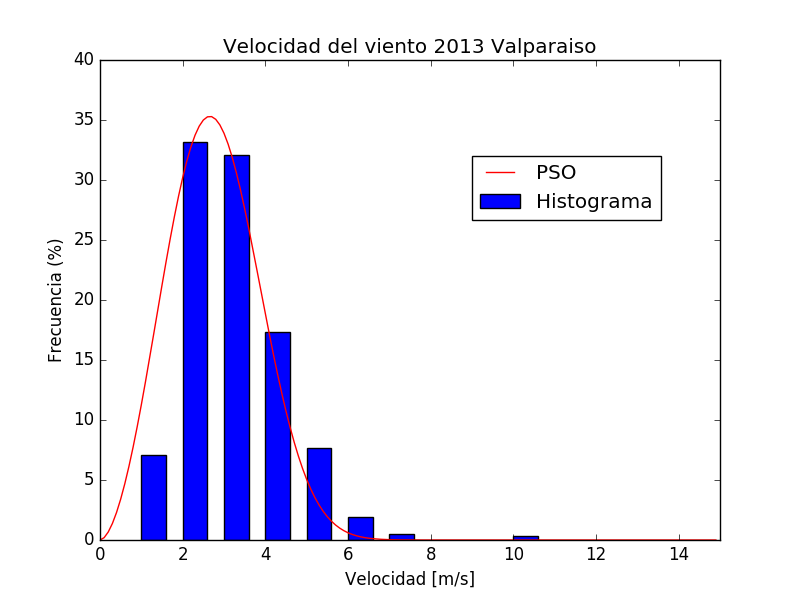
\includegraphics[width=0.4\textwidth]{figures/result_2013.png}
        }%
        \subfigure[PSO Valparaíso 2014.]{
            \label{fig:pso_valpo_14}
            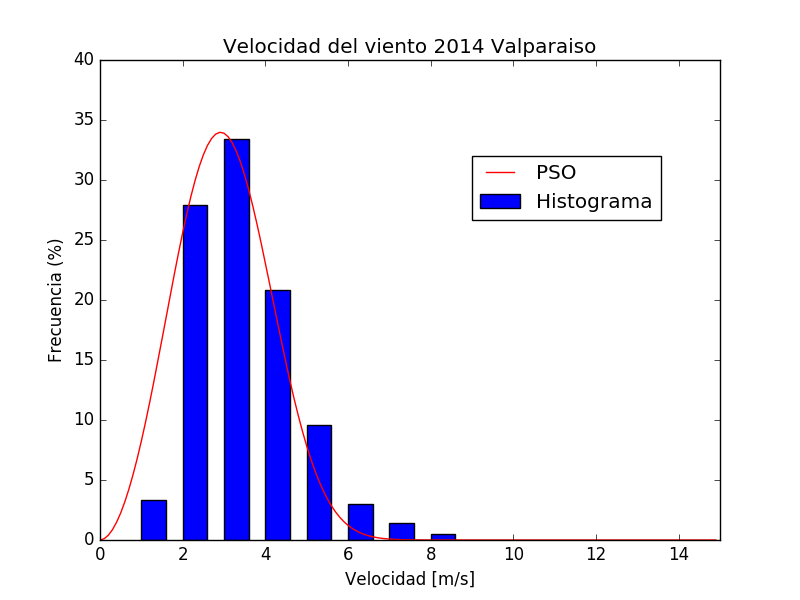
\includegraphics[width=0.4\textwidth]{figures/result_2014.png}
        }\\
        \subfigure[PSO Valparaíso 2015.]{
            \label{fig:pso_valpo_15}
            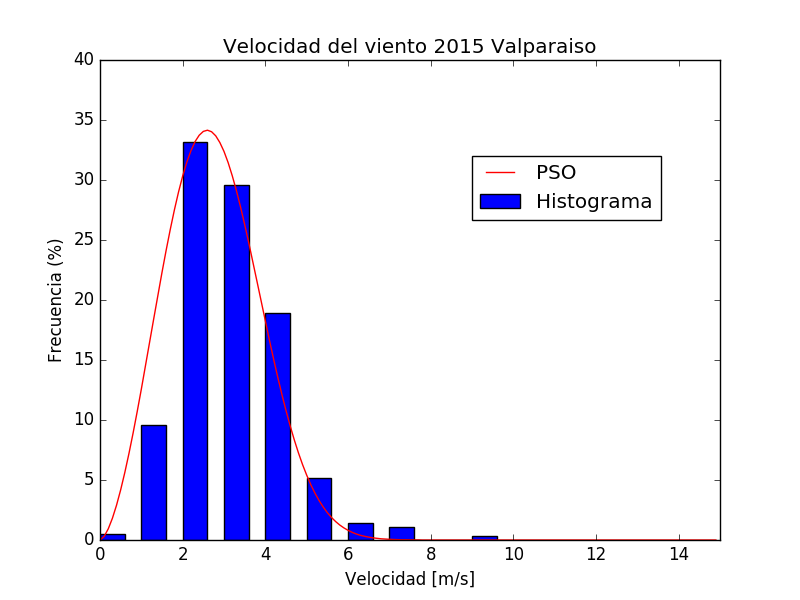
\includegraphics[width=0.4\textwidth]{figures/result_2015.png}
        }%
    \caption{Ajuste con PSO a datos del viento de Valparaíso.\\ Fuente: Elaboración Propia.}
    \label{fig:subfigures}
\end{figure}

\subsubsection{Experimento 2, datos de tres años y promedios diarios}
En este experimento se realizó el ajuste considerando los promedios diarios y un intervalo de tres años consecutivos. El gráfico \ref{fig:pso_valpo_15_14_13_lq}, muestra el resultado del ajuste con PSO y la configuración estándar de los demás experimentos, es decir, 100 iteraciones y 50 partículas. En este gráfico se aprecia que el ajuste no es bueno, a pesar de las cifras en la tabla \ref{table:stadistical_tests}, fila 4: PSO (Intento 1), dado que oscila bastante alrededor de las barras del histograma, por lo que se repite el experimento aumentando el número de partículas a 200 obteniendo el gráfico \ref{fig:pso_valpo_15_14_13}, con el cual se obtiene un ajuste más adecuado, además de mejorar los resultados de los test estadísticos (tabla \ref{table:stadistical_tests}, fila 5: PSO (Intento 2)).\\
\begin{figure}[ht!]
    \centering
        \subfigure[Buen ajuste PSO Valparaíso 2013.]{
            \label{fig:pso_valpo_15_14_13}
            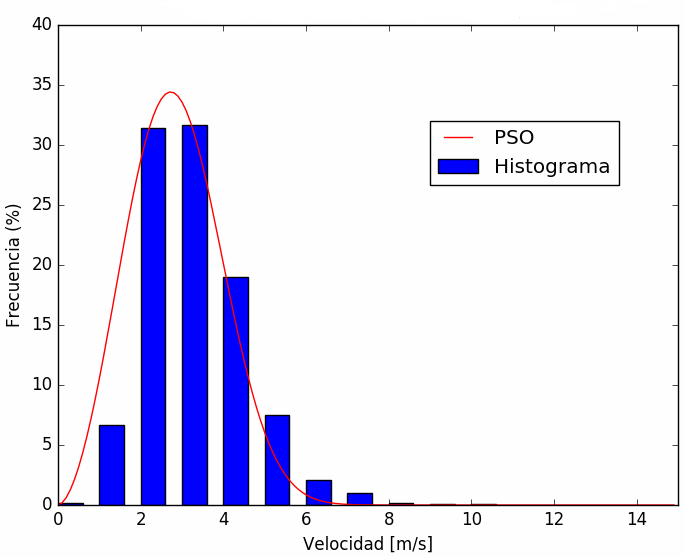
\includegraphics[width=0.4\textwidth]{figures/result_13-14-15.png}
        }%
        \subfigure[Mal ajuste PSO Valparaíso 2013.]{
            \label{fig:pso_valpo_15_14_13_lq}
            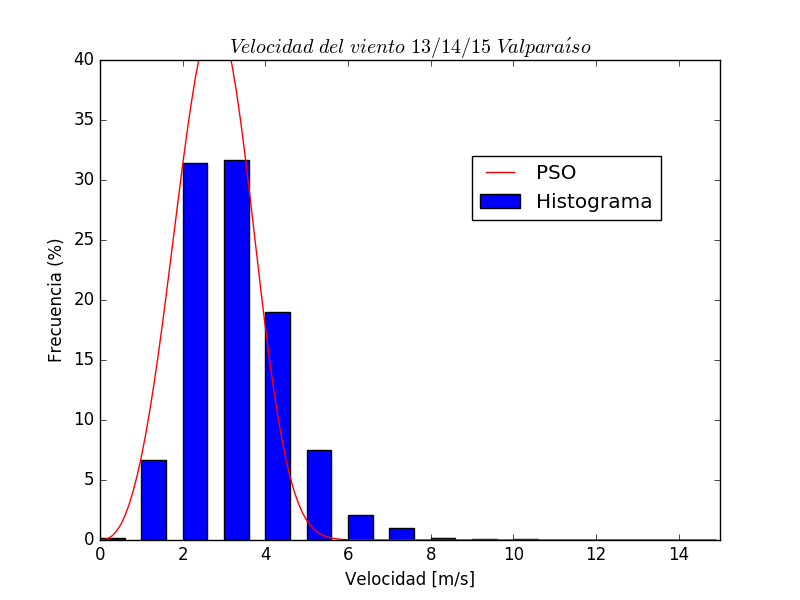
\includegraphics[width=0.4\textwidth]{figures/result_13-14-15_low_quality.png}
        }%
    \caption{Ajuste con PSO a datos Valparaíso 2015, 2014 y 2013, baja y buena calidad.\\ Fuente: Elaboración Propia.}
    \label{fig:subfigures}
\end{figure}

\subsubsection{Experimento 3, ajuste a datos anuales con resultados del experimento 2}
Los gráficos \ref{fig:pso_valpo_13_all_data}, \ref{fig:pso_valpo_14_all_data} y \ref{fig:pso_valpo_15_all_data} son ajustes de Weibull con los parámetros obtenidos en el experimento anterior. Es decir, la idea es evaluar el modelo general de los tres años versus el histograma de datos de cada año en particular.
El ajuste desde los resultados estadísticos (tabla \ref{table:stadistical_tests}), es levemente menos preciso que el modelo ajustado a cada año en particular, pero sigue siendo aceptable como posible opción a considerar.
\begin{figure}[ht!]
    \centering
    \subfigure[Velocidad viento Valparaíso 2013.]{
        \label{fig:pso_valpo_13_all_data}
        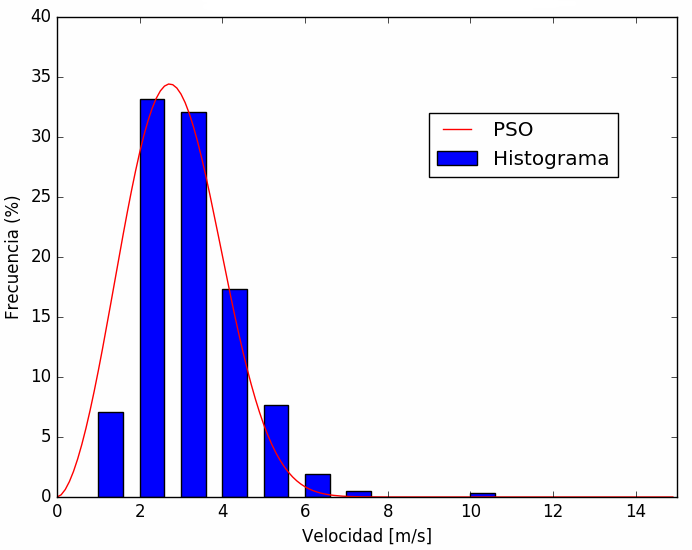
\includegraphics[width=0.4\textwidth]{figures/result_2013_fit_all_data.png}
    }%  
    \subfigure[Velocidad viento Valparaíso 2014.]{
        \label{fig:pso_valpo_14_all_data}
        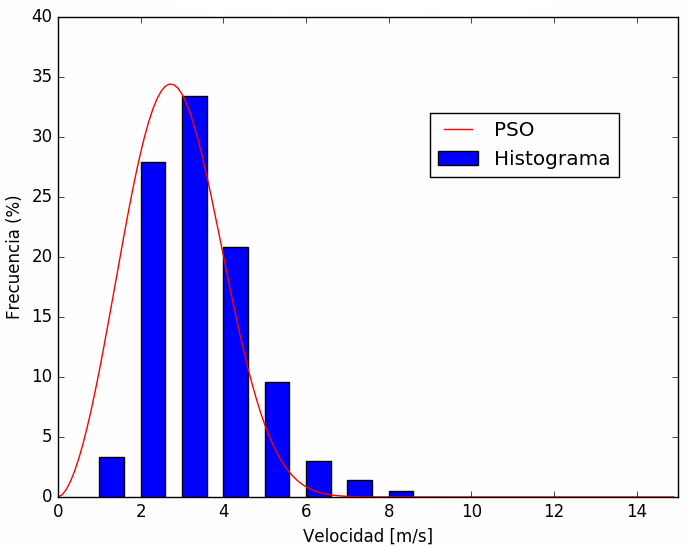
\includegraphics[width=0.4\textwidth]{figures/result_2014_fit_all_data.png}
    }\\   
    \subfigure[Velocidad viento Valparaíso 2015.]{
        \label{fig:pso_valpo_15_all_data}
        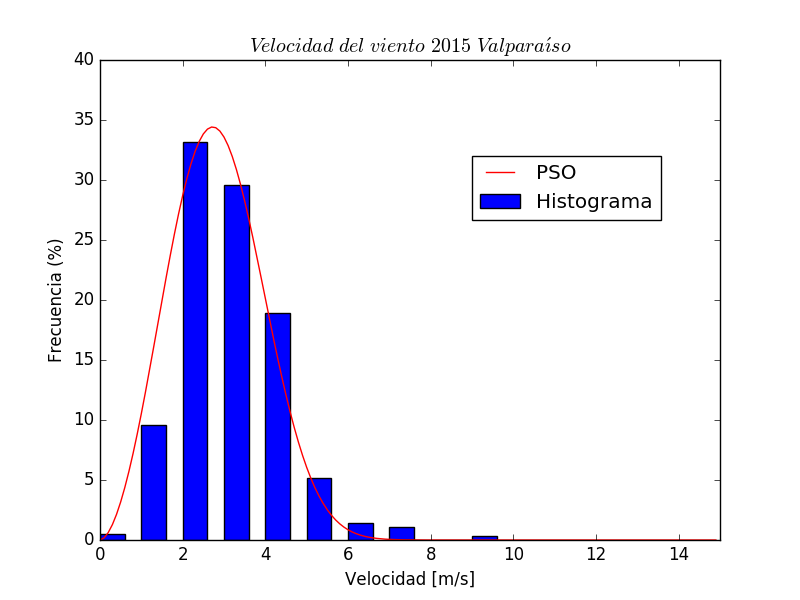
\includegraphics[width=0.4\textwidth]{figures/result_2015_fit_all_data.png}
    }%     

    \caption{Ajuste con PSO a registros del viento en Valparaíso (Con todos los datos).\\ Fuente: Elaboración Propia.}
    \label{fig:subfigures}
\end{figure}

\subsubsection{Experimento 4, ajuste a datos de tres meses y promedios diarios}
Es posible que se requiera un análisis más acotado, por ello los gráficos \ref{fig:pso_valpo_15_ene_mar}, \ref{fig:pso_valpo_15_abr_jun}, 
\ref{fig:pso_valpo_15_jul_sep}, \ref{fig:pso_valpo_15_oct_dic}, muestran un ajuste considerando un lapso de 3 meses para el año 2015, con el
que se demuestra que es posible definir cualquier intervalo (manteniendo como unidad de dato el promedio diario de velocidad del viento)
 y obtener un ajuste adecuado de los datos mediante la distribución de Weibull.

\begin{figure}[ht!]
    \centering
    \subfigure[Enero - Marzo.]{
        \label{fig:pso_valpo_15_ene_mar}
        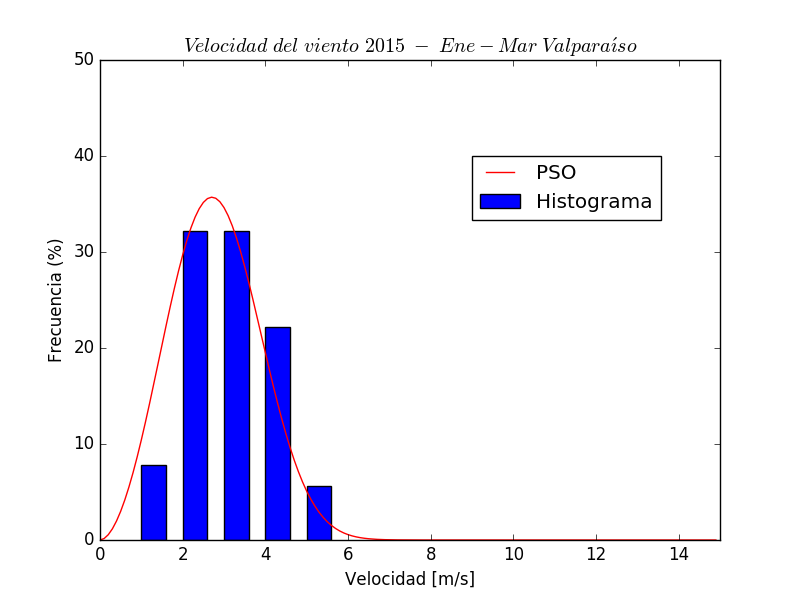
\includegraphics[width=0.4\textwidth]{figures/result_2015_Ene-Mar.png}
    }%  
    \subfigure[Abril - Junio.]{
        \label{fig:pso_valpo_15_abr_jun}
        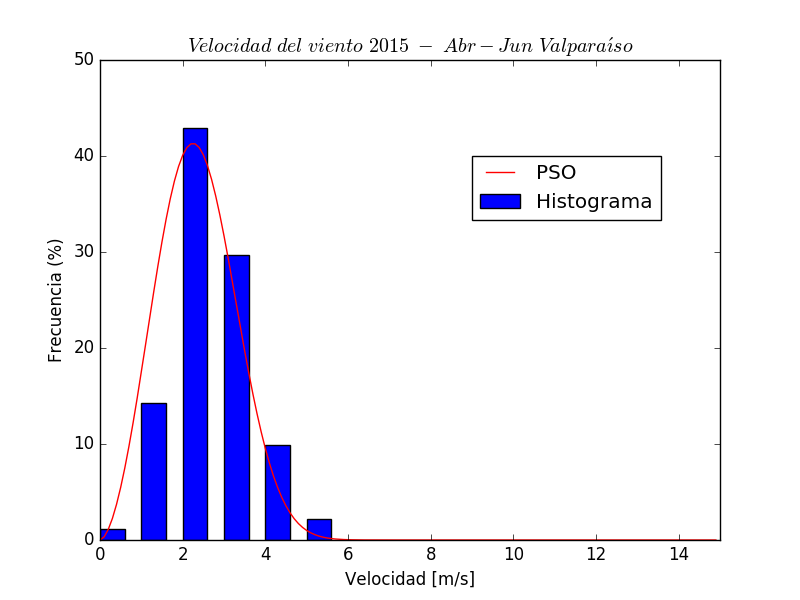
\includegraphics[width=0.4\textwidth]{figures/result_2015_Abr-Jun.png}
    }\\  
    \subfigure[Julio - Septiembre.]{
        \label{fig:pso_valpo_15_jul_sep}
        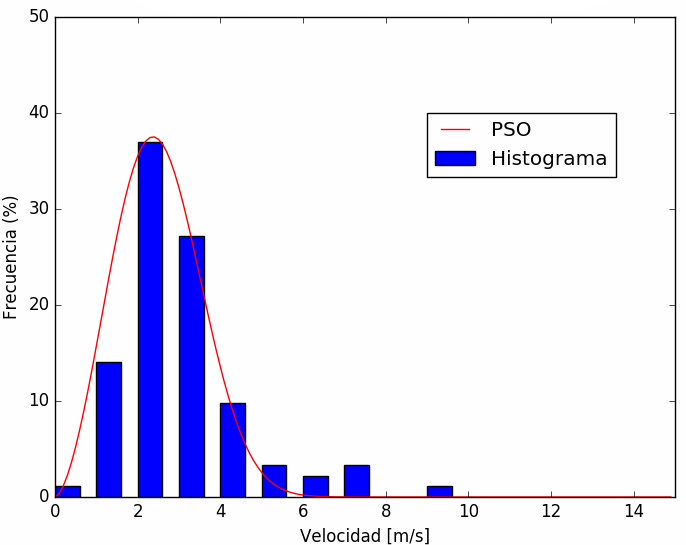
\includegraphics[width=0.4\textwidth]{figures/result_2015_Jul-Sep.png}
    }% 
    \subfigure[Octubre - Diciembre.]{
        \label{fig:pso_valpo_15_oct_dic}
        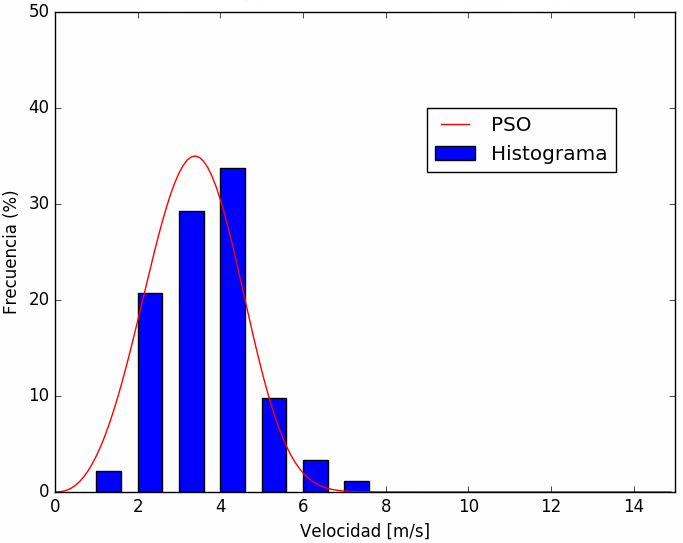
\includegraphics[width=0.4\textwidth]{figures/result_2015_Oct-Dic.png}
    }%  
    \caption{Ajuste con PSO a datos Valparaíso 2015, por rango de meses.\\ Fuente: Elaboración Propia.}
    \label{fig:subfigures}
\end{figure}

\subsubsection{Experimento 4, ajuste a datos año 2015 y datos brutos}
La razón de por qué se utiliza el promedio diario de los datos del viento para ajustar Weibull y no las mediciones puras (las mediciones tomadas cada 3 horas diariamente) es expuesta en el gráfico \ref{fig:pso_valpo_15_all_data}. La distribución de Weibull no se ajusta a una distribución de datos con más de un máximo, por lo que de requerirse un modelo para este caso se debe buscar otra distribución o modificar la distribución de Weibull. Es por ello que normalmente se utiliza un promedio del los datos, como se realiza en el trabajo de Farade \cite{Fadare08}.

\begin{figure}[ht!]
    \centering
    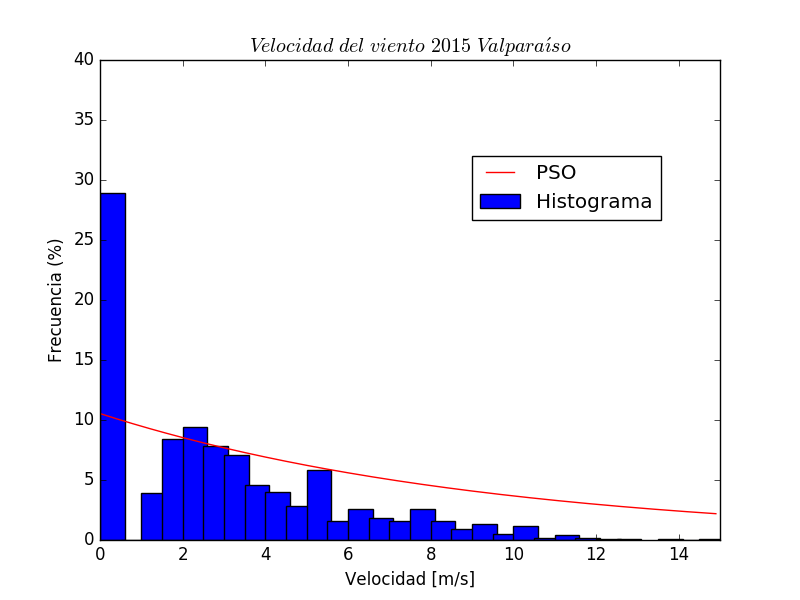
\includegraphics[width=0.4\textwidth]{figures/result_2015_all_data.png}
    \caption{Ajuste con PSO a datos (cifras puras) Valparaíso 2015, 2014, 2013}
    \vspace{-.25cm}
    \caption*{Fuente: Elaboración Propia.}
    \label{fig:pso_valpo_15_all_data}
\end{figure}

\subsubsection{Resumen de los experimentos}
\begin{table}[ht!]
    %\centering
    \caption{Tabla de tests estadísticos}
    \label{table:stadistical_tests}
    \resizebox{\textwidth}{!}{
    \begin{tabular}{|c|c|c|c|c|c|c|c|}
        \hline
        \textbf{\#} & \textbf{Método} & \textbf{Período} & \textbf{k} & \textbf{c} & \textbf{RMSE} & \textbf{r} & \textbf{RB}\\
        \hline
        1 & PSO & 2013 & 2.78 & 3.12 &0.0226585230791 & 0.984353070415 & 0.00197971468299\\
        2 & PSO & 2014 & 2.91 & 3.37 &0.0232779965263 & 0.982087745069 & 0.000754465101398\\
        3 & PSO & 2015 & 2.65 & 3.10 &0.0164721412159 & 0.992323803649 & 0.00302918178445\\
        \hline
        4 & PSO (Intento 1) & 2015-14-13 & 3.47 & 3.07 & 0.0360794587206 & 0.975240385258 & 0.000411212628513\\
        5 & PSO (Intento 2) & 2015-14-13 & 2.78 & 3.20 & 0.016175531561 & 0.994989105807 & 0.00190916669626\\
        \hline
        6 & PSO (Intento 2) & 2013 & 2.78 & 3.20 & 0.0240448436122 & 0.981963054492 & 0.00192186034284\\
        7 & PSO (Intento 2) & 2014 & 2.78 & 3.20 & 0.0301463089474 & 0.970662237238 & 8.89024791609e-05\\
        8 & PSO (Intento 2) & 2015 & 2.78 & 3.20 & 0.0202342934641 & 0.98662798667 & 0.00192175053173\\
        \hline
        9 & PSO & Ene-Mar & 2.85 & 3.15 & 0.0230380400157 & 0.982158006469 & 0.00641888742608\\
        10 & PSO & Abr-Jun & 2.76 & 2.65 & 0.0204300909755 & 0.993857185938 & 0.00303620481316\\
        11 & PSO & Jul-Sep & 2.66 & 2.83 & 0.0251002816356 & 0.985858767021 & 0.00443453471038\\
        12 & PSO & Oct-Dic & 3.40 & 3.75 & 0.0260278634297 & 0.978479679326 & 0.000716653529598\\
        \hline 
        13 & PSO (datos brutos) & 2015 & 1.00 & 9.49 & 0.0451794472583 & 0.751732944794 & 0.676094670465\\ 
        \hline
    \end{tabular}
    }   
\end{table}
\pagebreak
\subsection{Análisis de los resultados - dirección del viento}
\subsubsection{Experimento 1, pruebas iniciales}

En la figura \ref{fig:BAD_ADJUST} se puede observar un ajuste bastante distorsionado respecto al histograma de datos. Esto se debe a que la función objetivo del PSO evalúa la diferencia entre las frecuencias experimentales y las obtenidas teóricamente, por lo tanto, diferentes curvas pueden tener igual magnitud del área bajo la curva y por ende, la misma probabilidad con la que se obtiene la frecuencia teórica.\\
Por esto, es importante que el PSO busque mejorar la solución inicial en una vecindad cercana a esta, de manera de obtener una evolución como la que se aprecia en la figura \ref{fig:EV_SO}. Por ello, el algoritmo inicializa las partículas en la posición de la solución inicial encontrada más o menos una pequeña perturbación.   
\begin{figure}[ht!]
     \centering
        \subfigure[Ejemplo de mal ajuste, 2015.]{
            \label{fig:BAD_ADJUST}
            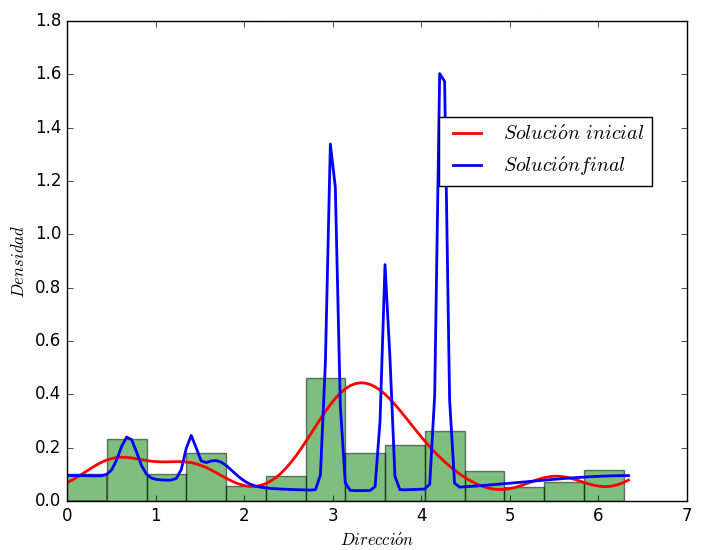
\includegraphics[width=0.4\textwidth]{figures/bad_adjust.png}
        }
        \subfigure[Evolucion de la solucion.]{
            \label{fig:EV_SOL}
            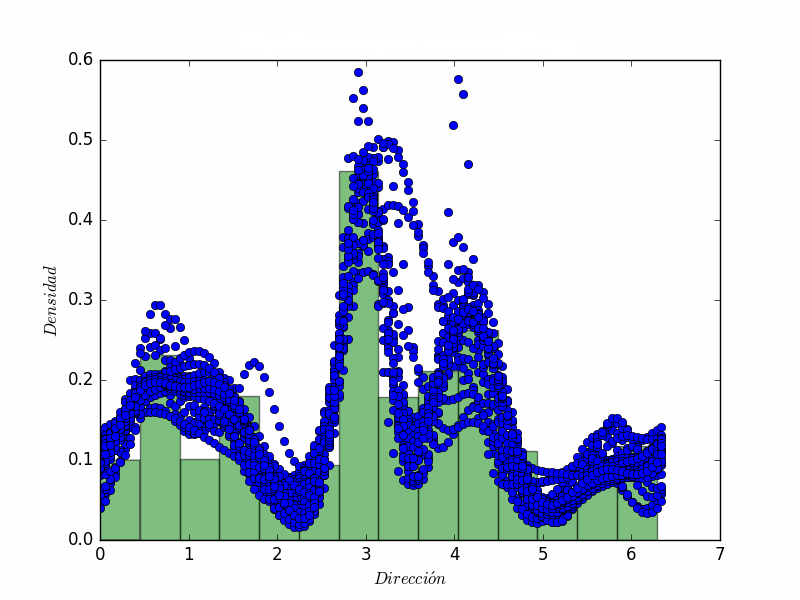
\includegraphics[width=0.4\textwidth]{figures/ev_solution.png}
        }%
    \caption{Pruebas iniciales.\\ Fuente: Elaboración propia.}
    \label{fig:subfigures}
\end{figure}

\subsubsection{Experimento 2, Ajustes anuales}
En este experimento se ajustan los vientos anualmente, en los años de los cuales se obtuvieron datos para este estudio, resultado la figura \ref{fig:SOL_13} para el 2013, la figura \ref{fig:SOL_14} para el 2014 y la figura \ref{fig:SOL_15} para el 2015.
Tal como se realiza en otros estudios \cite{Heckenbergerova15} \cite{Winddirelse15}, el ajuste de los datos de dirección del viento en un formato
de largo plazo, permite observar el comportamiento global de los vientos pudiendo evaluar la norma o generalidad en los datos registrados.
En las figuras referenciadas previamente se observa la evolución de la solución desde la aproximación inicial hasta la mejorada por el PSO.

\begin{figure}[ht!]
     \centering
        \subfigure[Solución inicial y final, 2015.]{
           \label{fig:SOL_15}
           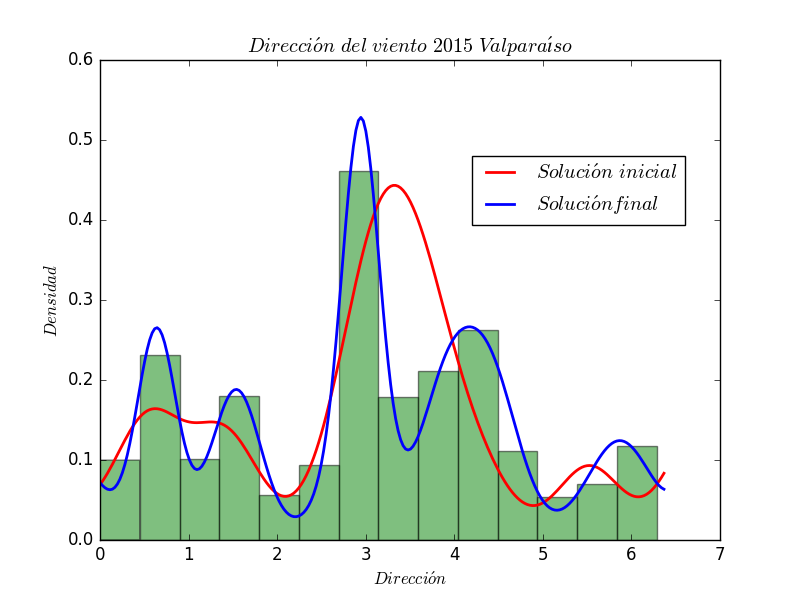
\includegraphics[width=0.4\textwidth]{figures/sol_ini_sol_fin.png}
        }
        \subfigure[Solución inicial y final, 2014.]{
            \label{fig:SOL_14}
            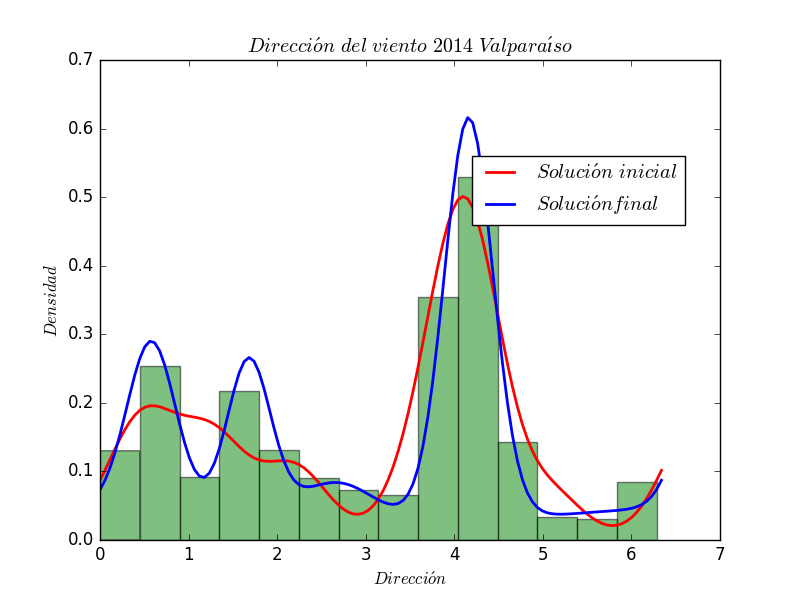
\includegraphics[width=0.4\textwidth]{figures/sol_ini_sol_fin_2014.png}
        }\\
         \subfigure[Solución inicial y final, 2013.]{
            \label{fig:SOL_13}
            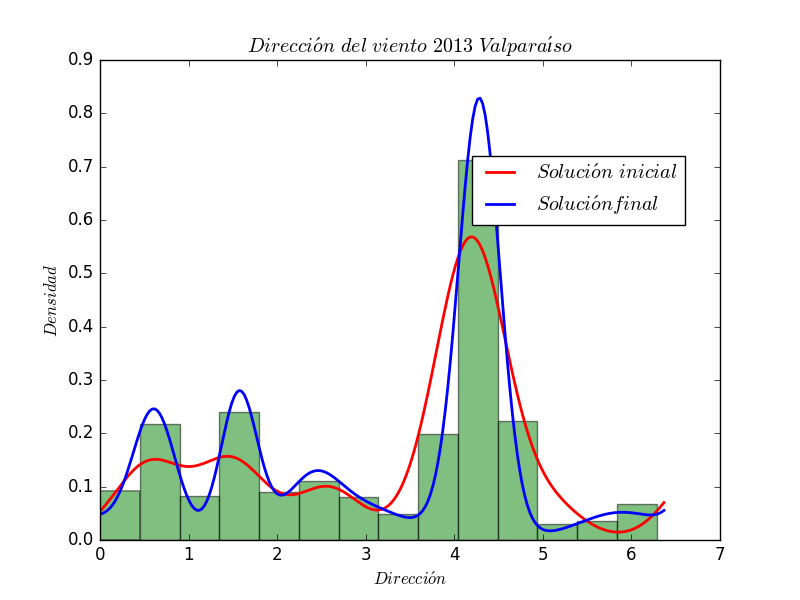
\includegraphics[width=0.4\textwidth]{figures/sol_ini_sol_fin_2013.png}
        }
    \caption{Graficos de ajustes anuales.\\ Fuente: Elaboración propia.}
    \label{fig:subfigures}
\end{figure}

\subsubsection{Experimento 3, Ajustes de meses acumulados}
Similar al ejercicio anterior, los gráficos agrupados en \ref{fig:PLOT_MONTHS_ALL_1} y \ref{fig:PLOT_MONTHS_ALL_2}, permiten visualizar el ajuste de los datos del viento por meses. En este caso se agruparon los datos de los tres años escogidos por cada mes, es decir, la figura \ref{fig:PLOT_SOL_ENERO}, por ejemplo, contiene los datos del mes de enero de los años 2013, 2014 y 2015.\\
Se puede observar que algunos gráficos muestran un mejor ajuste que otros, a pesar del correcto valor obtenido en la función objetivo como se expresa posteriormente en la tabla \ref{table:stadistical_tests_direction}. Esto se debe a que probablemente la solución se escapa más de los deseado de la solución inicial. 
\begin{figure}[ht!]
    \begin{center}
         %%MONTHS  
        \subfigure[Solución inicial y final, Enero.]{
            \label{fig:PLOT_SOL_ENERO}
            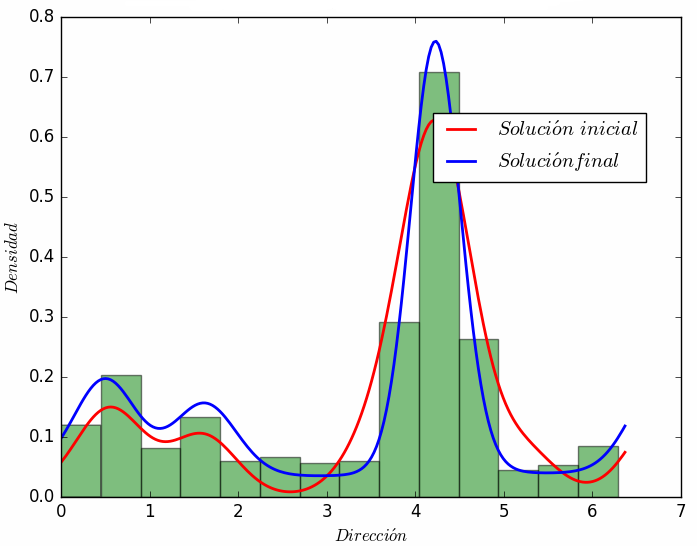
\includegraphics[width=0.4\textwidth]{figures/sol_ini_sol_fin_ENERO.png}
        }
         \subfigure[Solución inicial y final, Febrero.]{
            \label{fig:PLOT_SOL_FEBRERO}
            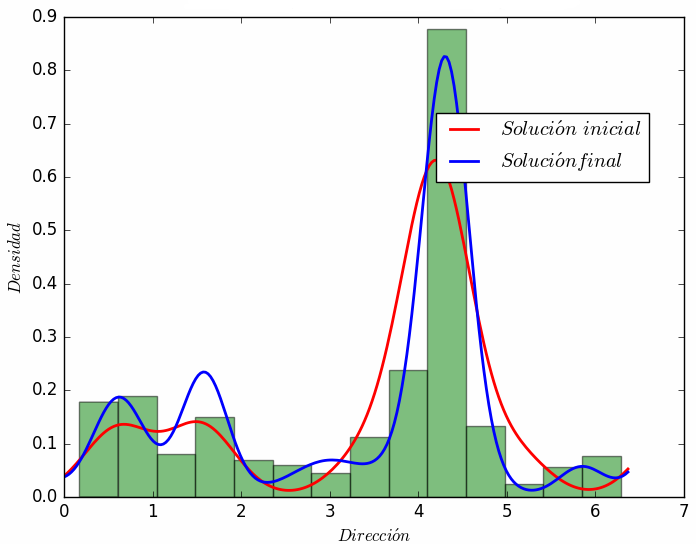
\includegraphics[width=0.4\textwidth]{figures/sol_ini_sol_fin_FEBRERO.png}
        }
          \subfigure[Solución inicial y final, Marzo.]{
            \label{fig:PLOT_SOL_MARZO}
            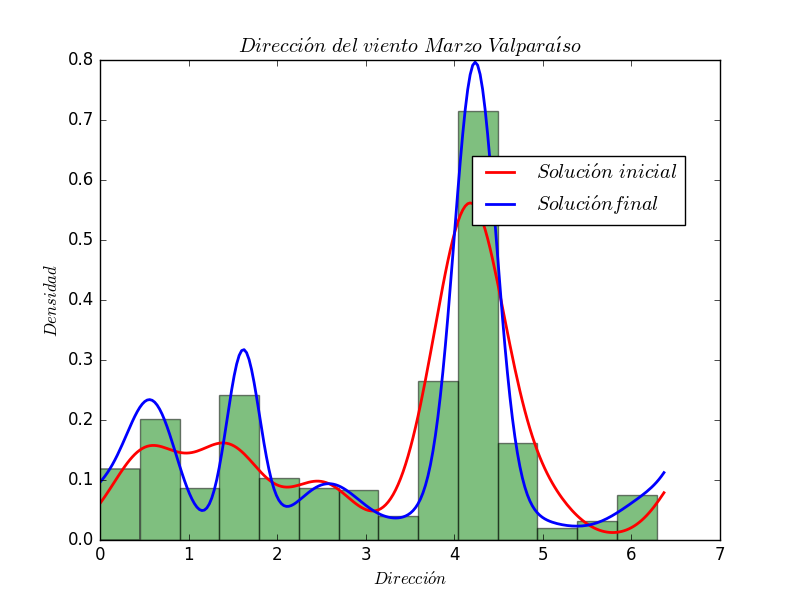
\includegraphics[width=0.4\textwidth]{figures/sol_ini_sol_fin_MARZO.png}
        }\\
         \subfigure[Solución inicial y final, Abril.]{
            \label{fig:PLOT_SOL_ABRIL}
            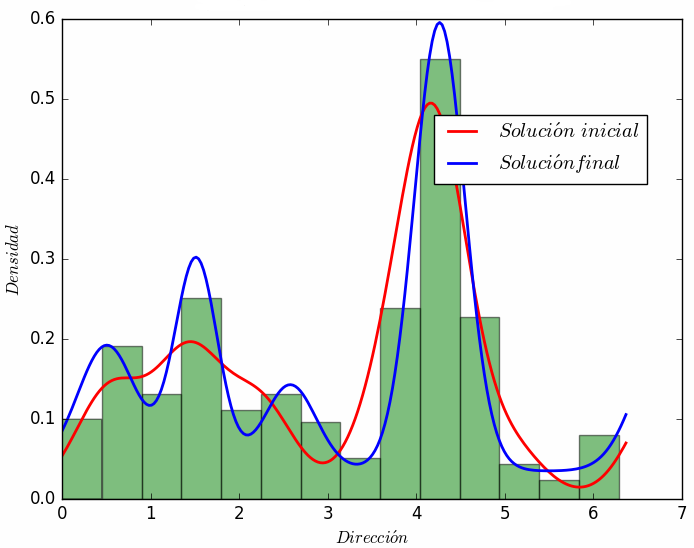
\includegraphics[width=0.4\textwidth]{figures/sol_ini_sol_fin_ABRIL.png}
        }
          \subfigure[Solución inicial y final, Mayo.]{
            \label{fig:PLOT_SOL_MAYO}
            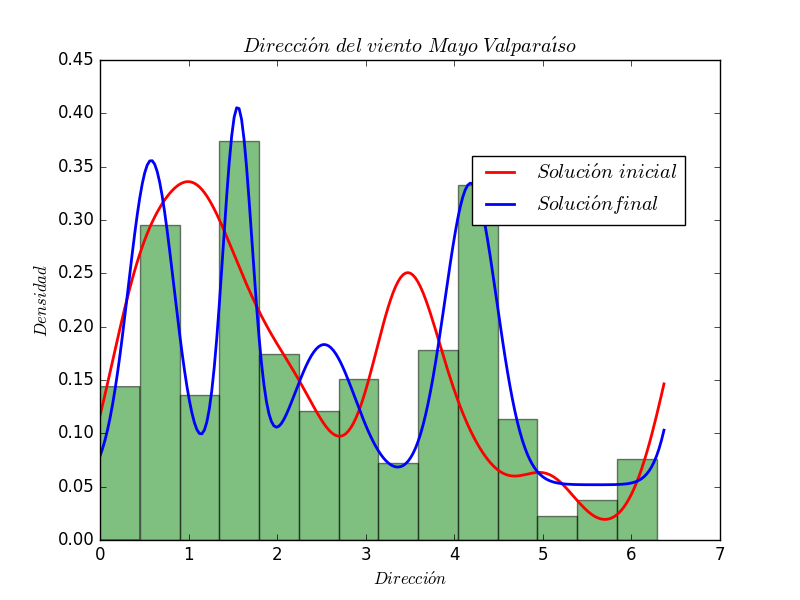
\includegraphics[width=0.4\textwidth]{figures/sol_ini_sol_fin_MAYO.png}
        }
         \subfigure[Solución inicial y final, Junio.]{
            \label{fig:PLOT_SOL_JUNIO}
            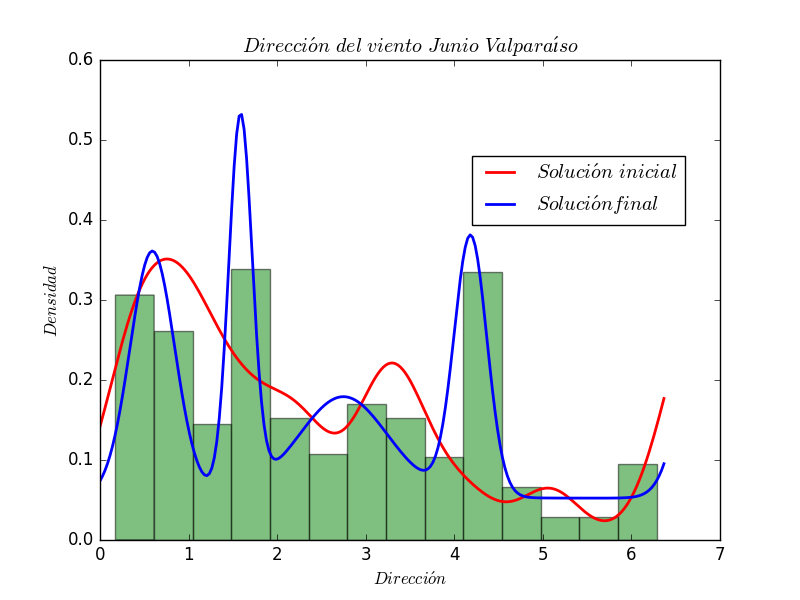
\includegraphics[width=0.4\textwidth]{figures/sol_ini_sol_fin_JUNIO.png}
        }
\end{center}
    \caption{Gráficos de ajuste de MVM por meses.\\ Fuente: Elaboración propia.}
    \label{fig:PLOT_MONTHS_ALL_1}
\end{figure}

\begin{figure}[ht!]
    \begin{center}
        \subfigure[Solución inicial y final, Julio.]{
            \label{fig:PLOT_SOL_JULIO}
            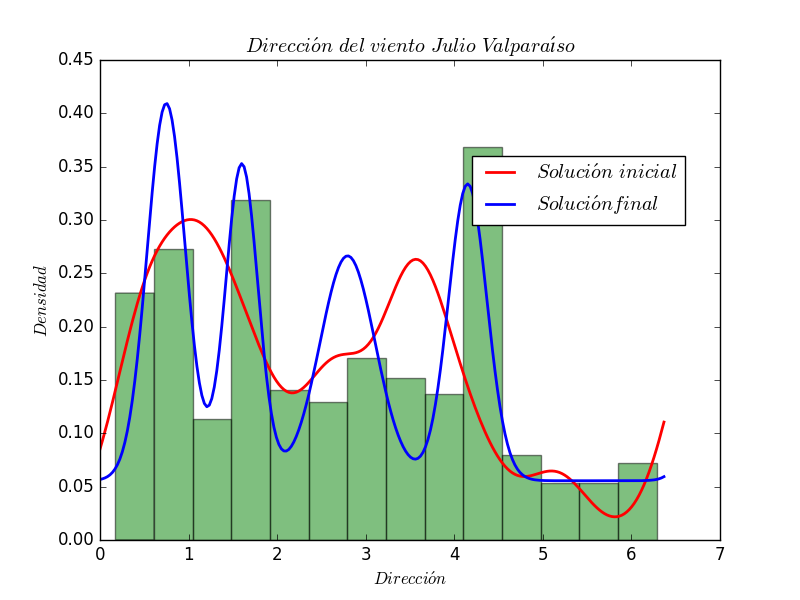
\includegraphics[width=0.4\textwidth]{figures/sol_ini_sol_fin_JULIO.png}
        }
         \subfigure[Solución inicial y final, Agosto.]{
            \label{fig:PLOT_SOL_AGOSTO}
            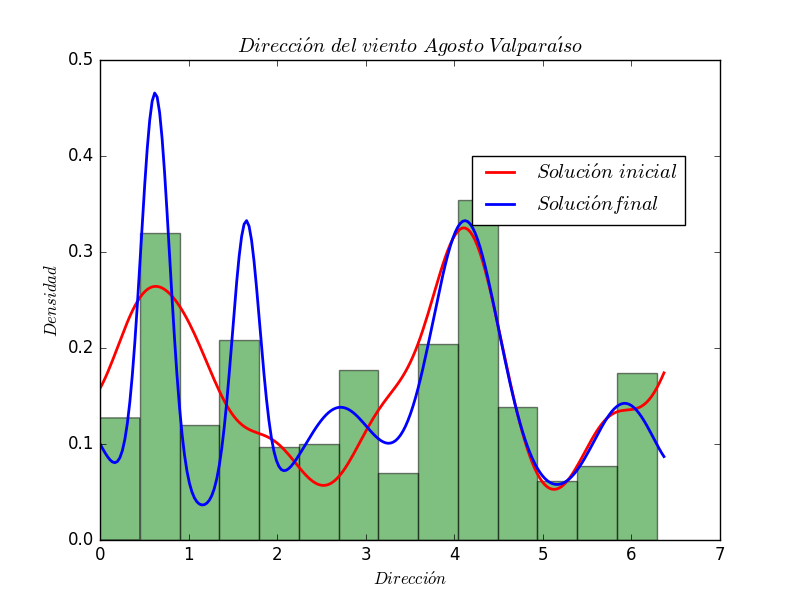
\includegraphics[width=0.4\textwidth]{figures/sol_ini_sol_fin_AGOSTO.png}
        }
          \subfigure[Solución inicial y final, Septiembre.]{
            \label{fig:PLOT_SOL_SEPTIEMBRE}
            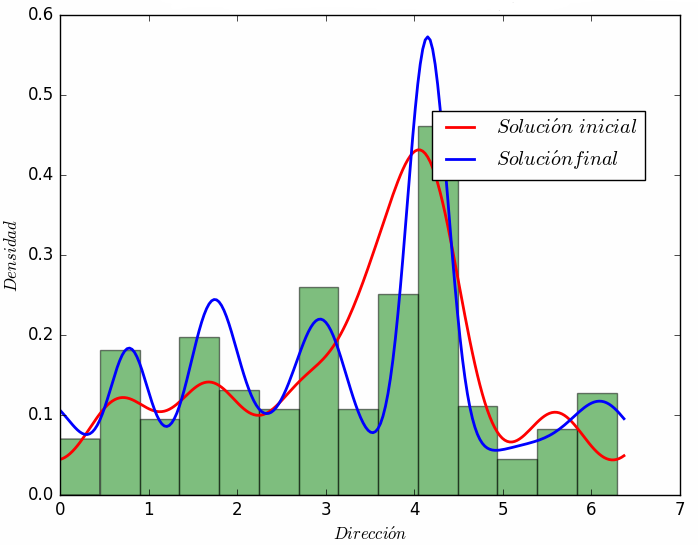
\includegraphics[width=0.4\textwidth]{figures/sol_ini_sol_fin_SEPTIEMBRE.png}
        }\\
         \subfigure[Solución inicial y final, Octubre.]{
            \label{fig:PLOT_SOL_OCTUBRE}
            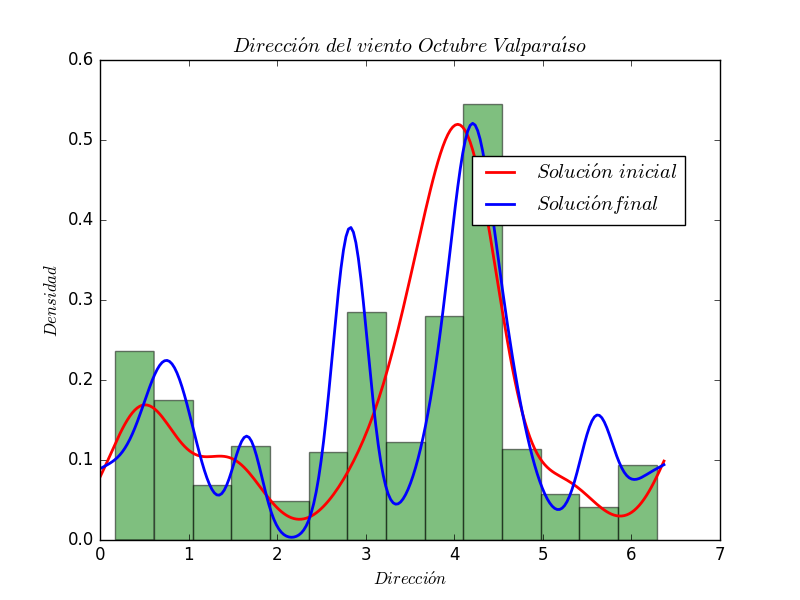
\includegraphics[width=0.4\textwidth]{figures/sol_ini_sol_fin_OCTUBRE.png}
        }
          \subfigure[Solución inicial y final, Noviembre.]{
            \label{fig:PLOT_SOL_NOVIEMBRE}
            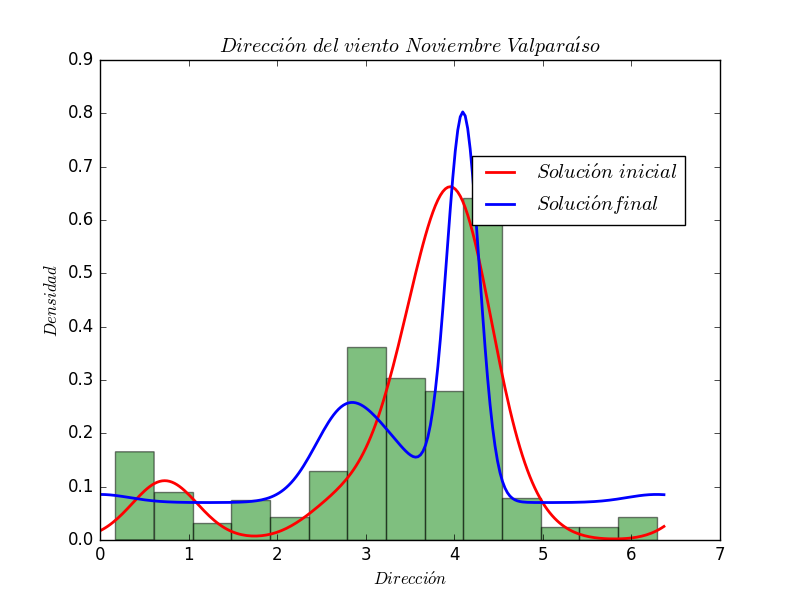
\includegraphics[width=0.4\textwidth]{figures/sol_ini_sol_fin_NOVIEMBRE.png}
        }
         \subfigure[Solución inicial y final, Diciembre.]{
            \label{fig:PLOT_SOL_DICIEMBRE}
            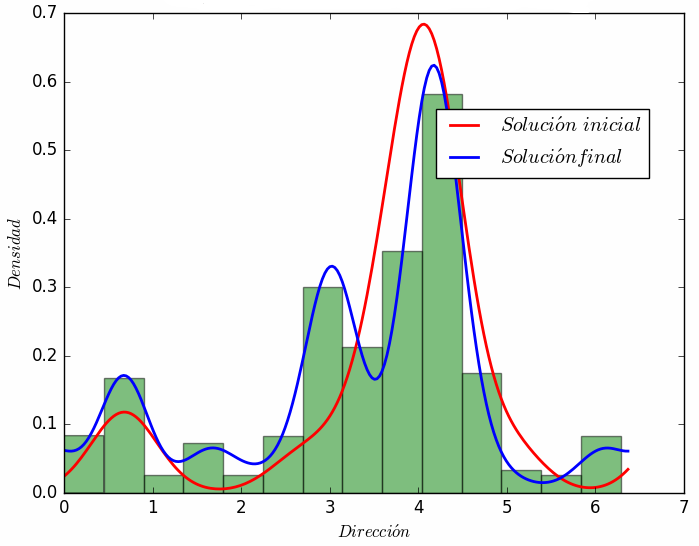
\includegraphics[width=0.4\textwidth]{figures/sol_ini_sol_fin_DICIEMBRE.png}
        }

    \end{center}
    \caption{Gráficos de ajuste de MVM por meses.\\ Fuente: Elaboración propia.}
    \label{fig:PLOT_MONTHS_ALL_2}
\end{figure}

\subsubsection{Experimento 4, Ajuste por meses, visualización en coordenadas polares}
En las figuras agrupadas \ref{fig:PLOT_MONTHS_1} y \ref{fig:PLOT_MONTHS_2} se aprecia una visualización más interesante. Allí se puede ver de forma más intuitiva las direcciones dominantes del viento, relativas al sistema de referencia utilizado en meteorología conocido comúnmente como la rosa de los vientos \cite{RosaViento}. En el mes de Enero \ref{polar_ene_2015}\ref{polar_ene_2014}\ref{polar_ene_2013}, los vientos parecen provenir principalmente desde el sur-oeste, mientras que en Mayo \ref{polar_may_2015}\ref{polar_may_2014}\ref{polar_may_2013} no es tan fija la fuente de los vientos, proveniendo desde el nor-este y el sur principalmente. En Septiembre \ref{polar_sep_2015}\ref{polar_sep_2014}\ref{polar_sep_2013}, vuelve a inclinarse la funtes de los vientos hacia el sur y sur-oeste.
\begin{figure}[ht!]
    \begin{center}
        \subfigure[Dirección enero 2015.]{
            \label{fig:polar_ene_2015}
            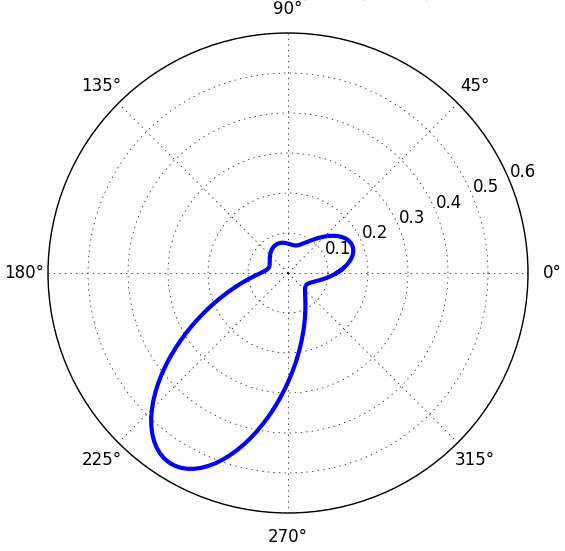
\includegraphics[width=0.4\textwidth]{figures/direction_enero_2015.png}
        }
         \subfigure[Dirección enero 2014.]{
            \label{fig:polar_ene_2014}
            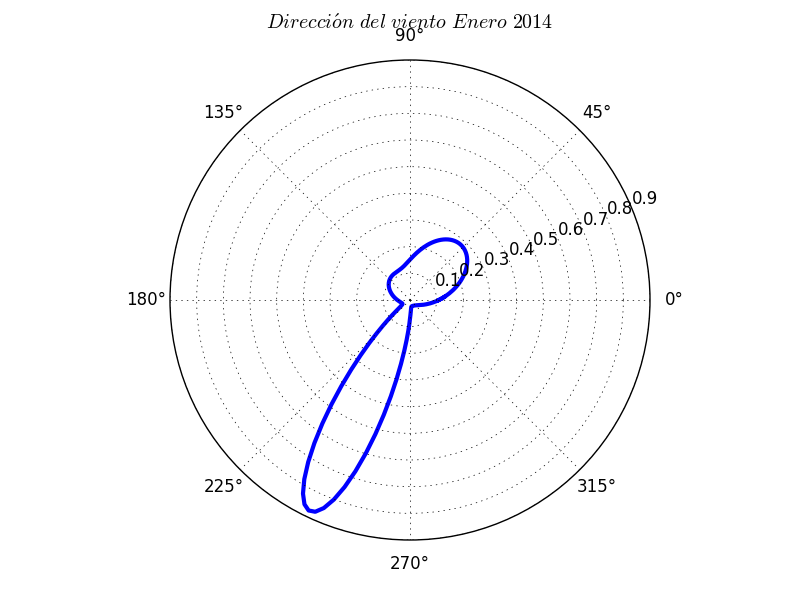
\includegraphics[width=0.4\textwidth]{figures/direction_enero_2014.png}
        }\\
         \subfigure[Dirección enero 2013.]{
            \label{fig:polar_ene_2013}
            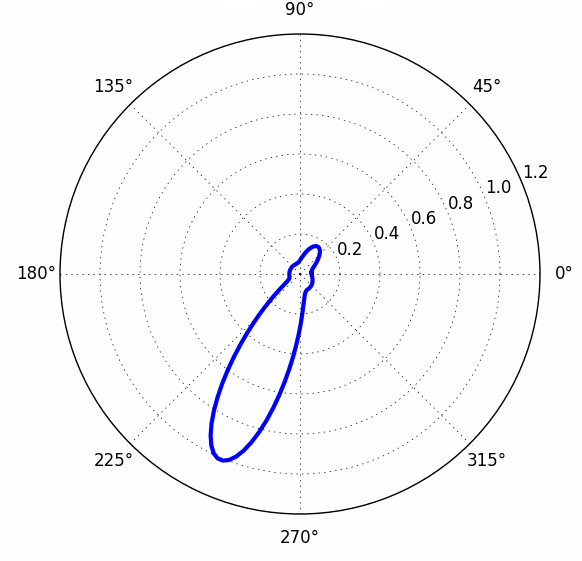
\includegraphics[width=0.4\textwidth]{figures/direction_enero_2013.png}
        }
         \subfigure[Dirección mayo 2015.]{
            \label{fig:polar_may_2015}
            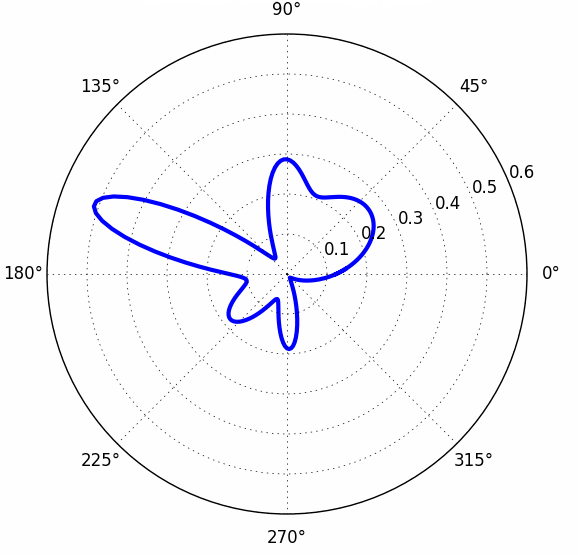
\includegraphics[width=0.4\textwidth]{figures/direction_mayo_2015.png}
        }\\
         \subfigure[Dirección mayo 2014.]{
            \label{fig:polar_may_2014}
            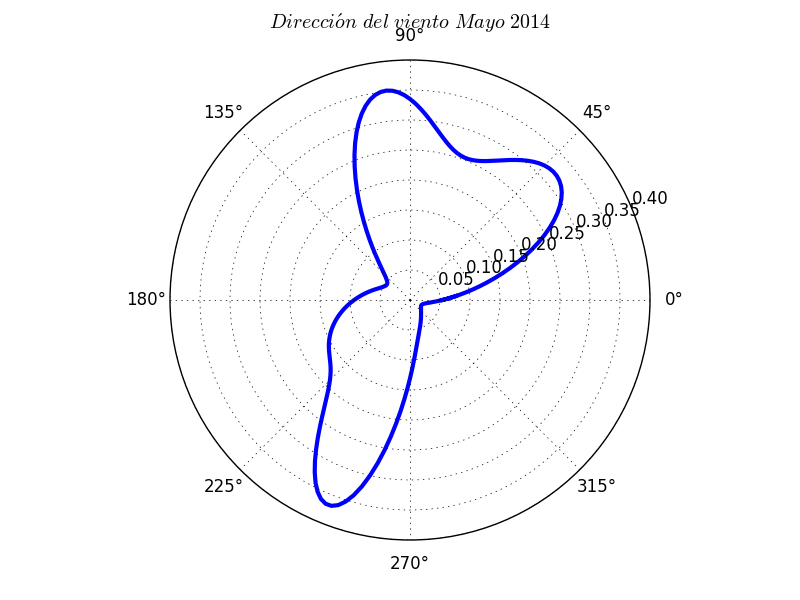
\includegraphics[width=0.4\textwidth]{figures/direction_mayo_2014.png}
        }
         \subfigure[Dirección mayo 2013.]{
            \label{fig:polar_may_2013}
            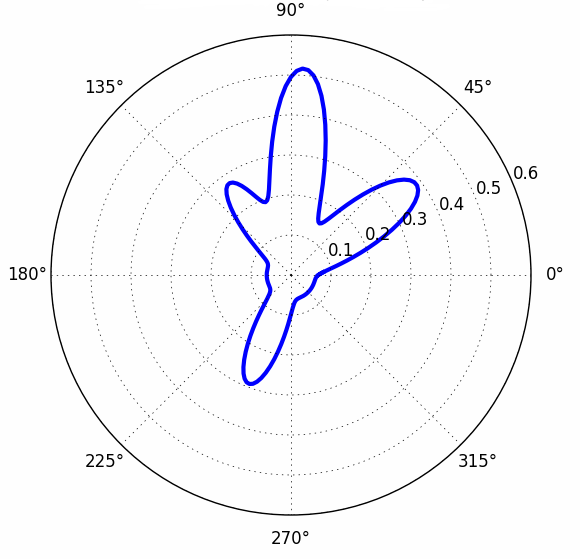
\includegraphics[width=0.4\textwidth]{figures/direction_mayo_2013.png}
        }
    \end{center}
    \caption{Gráficos de ajuste por meses en coordenadas polares.\\ Fuente: Elaboración propia.}
    \label{fig:PLOT_MONTHS_1}
\end{figure}

\begin{figure}[ht!]
    \begin{center}
        \subfigure[Dirección septiembre 2015.]{
            \label{fig:polar_sep_2015}
            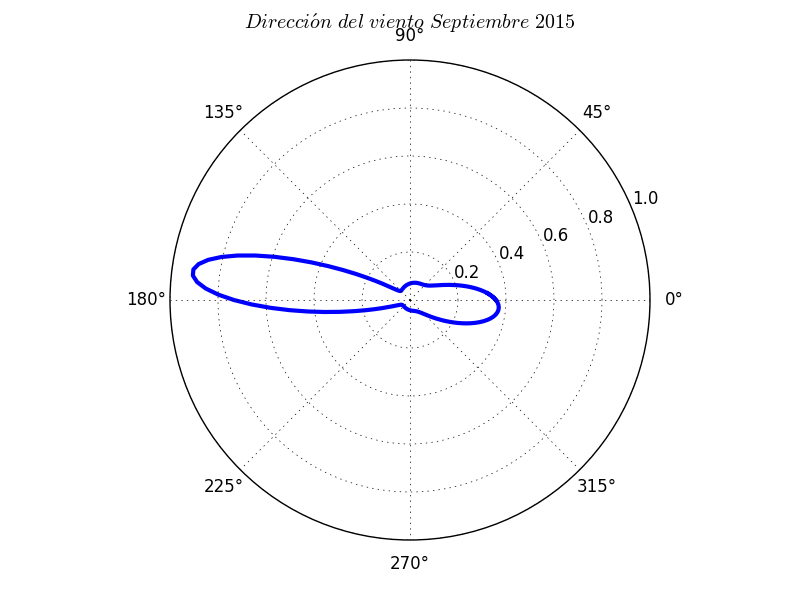
\includegraphics[width=0.4\textwidth]{figures/direction_septiembre_2015.png}
        }
         \subfigure[Dirección septiembre 2014.]{
            \label{fig:polar_sep_2014}
            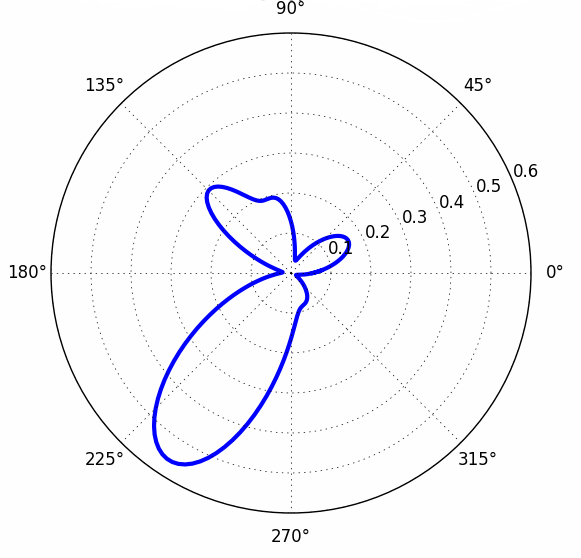
\includegraphics[width=0.4\textwidth]{figures/direction_septiembre_2014.png}
        }\\
         \subfigure[Dirección septiembre 2013.]{
            \label{fig:polar_sep_2013}
            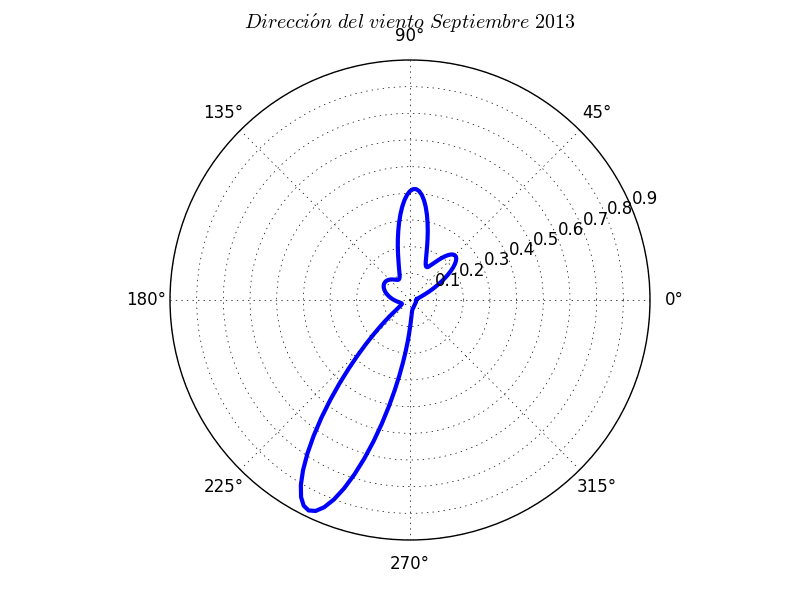
\includegraphics[width=0.4\textwidth]{figures/direction_septiembre_2013.png}
        }
    \end{center}    
    \caption{Gráficos de ajuste por meses en coordenadas polares.\\ Fuente: Elaboración propia.}
    \label{fig:PLOT_MONTHS_1}
\end{figure}

\subsubsection{Resumen de los experimentos}
\begin{table}[ht!]
    %\centering
    \caption{Tabla de tests estadísticos}
    \label{table:stadistical_tests_direction}
    \resizebox{\textwidth}{!}{
    \begin{tabular}{|c|c|c|c|c|c|c|c|c|}
        \hline
        \textbf{Periodo de tiempo} & \textbf{PSI} & \textbf{PSF1} & \textbf{PSF2} & \textbf{Tiempo 1} & \textbf{Tiempo 2} & \textbf{Iteraciones 1} & \textbf{Iteraciones 2} & \textbf{Cantidad datos}\\
        \hline
        2015            & 461.834005    & -             & 251.376863    & -             & 38m46.168s    & -     & 50500 & 2076 \\
        2015            & 461.834005    & 21.580166     & 234,977200    & 8m5.748s      & 47m47.136s    & 9005  & 50500 & 2076 \\
        2014            & 301.12834005  & 19.869808     & 56,579260     & 20m37.844s    & 46m23.256s    & 29494 & 50500 & 2499 \\ 
        2013            & 424.247097    & 20.76838      & 69,531194     & 11m41.128s    & 48m23.724s    & 16778 & 50500 & 2346 \\
        \hline
        Enero           & 144.420285    & 20.890711     & 22,180797     & 0m3.332s      & 25m37.239s    & 86    & 27276 & 633 \\
        Febrero         & 130.397909    & 19.450824     & 22,271337     & 0m12.260s     & 0m07.152s     & 288   & 134   & 567\\
        Marzo           & 104.544257    & 18.610565     & 22,310005     & 0m3.124s      & 0m13.384s     & 49    & 228   & 564 \\
        Abril           & 74.974500     & 21.135048     & 22,256276     & 0m12.564s     & 17m58.456s    & 192   & 18544 & 559 \\
        Mayo            & 243.656241    & 21.650182     & 81,752196     & 1m6.924s      & 42m59.612s    & 1237  & 50000 & 589 \\
        Junio           & 286.308891    & 21.018451     & 188,91869     & 1m42.996s     & 40m52.584s    & 1989  & 50000 & 554 \\
        Julio           & 177.338315    & 22.064056     & 31,393105     & 0m17.888s     & 45m48.368s    & 315   & 50000 & 604 \\
        Agosto          & 79.579614     & 21.940013     & 22,170518     & 0m12.940s     & 40m26.344s    & 202   & 41204 & 578 \\
        Septiembre      & 92.775196     & 21.313293     & 22,319598     & 0m1.776s      & 0m1.732s      & 27    & 166   & 541 \\
        Octubre         & 188.149963    & 21.810323     & 37,502260     & 0m45.356s     & 42m56.496s    & 825   & 50000 & 564 \\
        Noviembre       & 363.902142    & 26.25178      & 88,168226     & 42m21.400s    & 42m53.668s    & 50500 & 50000 & 582 \\
        Diciembre       & 335.286306    & 22.300924     & 37,814759     & 9m56.148s     & 43m52.916s    & 11640 & 50000 & 586 \\
        \hline 
        Enero 2015      & 42.941029     & 16.340722     & 18,773471     & 0m4.108s      & 0m0.196s      & 61    & 10    & 220 \\
        Enero 2014      & 68.102447     & 20.683871     & 21,604465     & 0m1.872s      & 0m0.728s      & 29    & 126   & 206 \\
        Enero 2013      & 194.988635    & 19.319721     & 24,860318     & 0m0.448s      & 46m29.220s    & 6     & 50000 & 207 \\
        Mayo 2015       & 60.843802     & 17.998473     & 26,693766     & 0m2.300s      & 41m53.804s    & 39    & 50000 & 173 \\
        Mayo 2014       & 142.856664    & 20.943375     & 20,483982     & 0m4.832s      & 0m0.3576s     & 82    & 50    & 213 \\
        Mayo 2013       & 135.687704    & 20.8897       & 22,346281     & 0m5.312s      & 0m1.044s      & 97    & 2089  & 203 \\
        Septiembre 2015 & 77.411834     & 21.293589     & 25,541457     & 0m8.420s      & 41m48.732s    & 137   & 50000 & 140 \\
        Septiembre 2014 & 19.563136     & 18.247167     & 15,869938     & 0m0.084s      & 0m0.036s      & 1     & 1     & 200 \\
        Septiembre 2013 & 68.904049     & 16.617326     & 21,890982     & 0m0.388s      & 0m0.980s      & 5     & 150   & 201 \\
        \hline  
    \end{tabular}
    }   
\end{table}
La tabla \ref{table:stadistical_tests_direction} muestra un resumen de los resultados obtenidos al ajustar la distribución de probabilidad \emph{von Mises distribution} en diferentes subconjuntos de tiempo de los datos colectados en los años 2013, 2014 y 2015. La tabla está organizada como sigue a continuación. La estrategia 1 hace referencia a la propuesta realizada en este trabajo, mientras que la estrategia 2 es la seguida en el trabajo de Heckenbergerova et al. \cite{Heckenbergerova15}, la cual consta simplemente de la definición de parámetros fijos para el PSO.
\begin{enumerate}
    \item \emph{Periodo de tiempo}: Rango de tiempo donde se consideraron los datos para el ajuste.
    \item \emph{PSI}: Puntaje solución inicial, es decir, el valor obtenido al evaluar la solución inicial en la función objetivo.
    \item \emph{PSF1}: Puntaje solución final 1, se refiere a la solución obtenida por el PSO al utilizar la estrategia explicada en \ref{eq:VariationParameters_new}.
    \item \emph{PSF2}:  Puntaje solución final 2, se refiere a la solución obtenida por el PSO al utilizar la estrategia tradicional.
    \item \emph{Tiempo 1}: Tiempo empleado por el PSO con la estrategia 1 \ref{eq:VariationParameters_new}. 
    \item \emph{Tiempo 2}: Tiempo empleado por el PSO con la estrategia 2. 
    \item \emph{Iteraciones 1}: Iteraciones empleadas por el PSO con la estrategia 1 \ref{eq:VariationParameters_new}. 
    \item \emph{Iteraciones 2}: Iteraciones empleadas por el PSO con la estrategia 2. 
    \item \emph{Cantidad datos}: Cantidad de datos utilizados en el ajuste.
\end{enumerate}

\begin{figure}[ht!]
    \begin{center}
        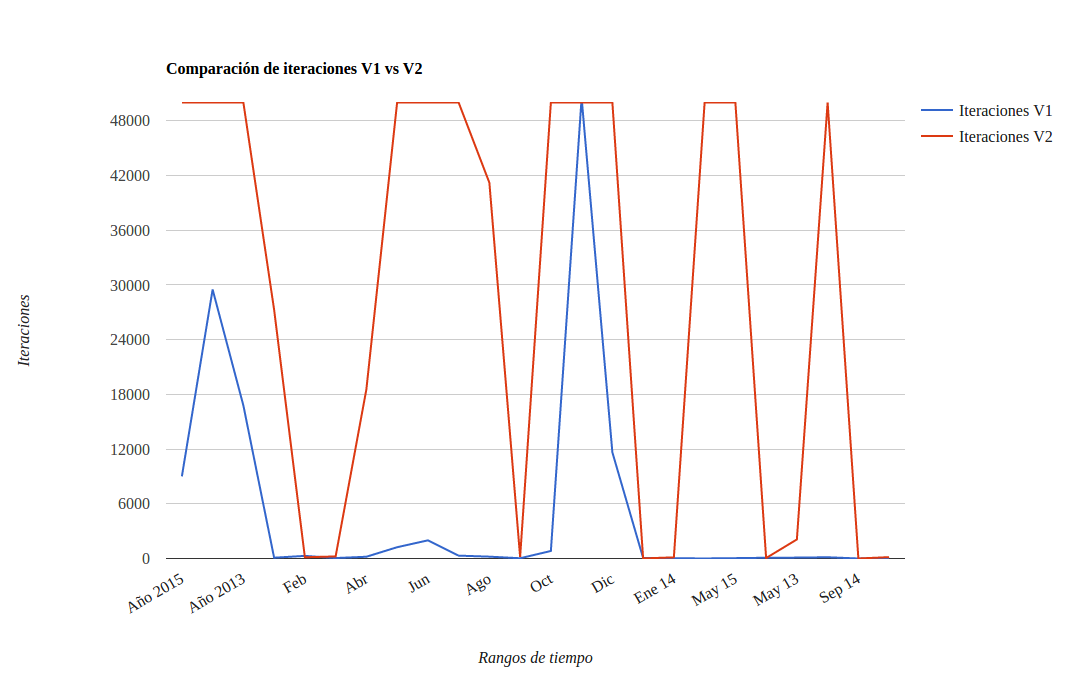
\includegraphics[width=\textwidth]{figures/comp_v1_v2_iteraciones.png}
       
        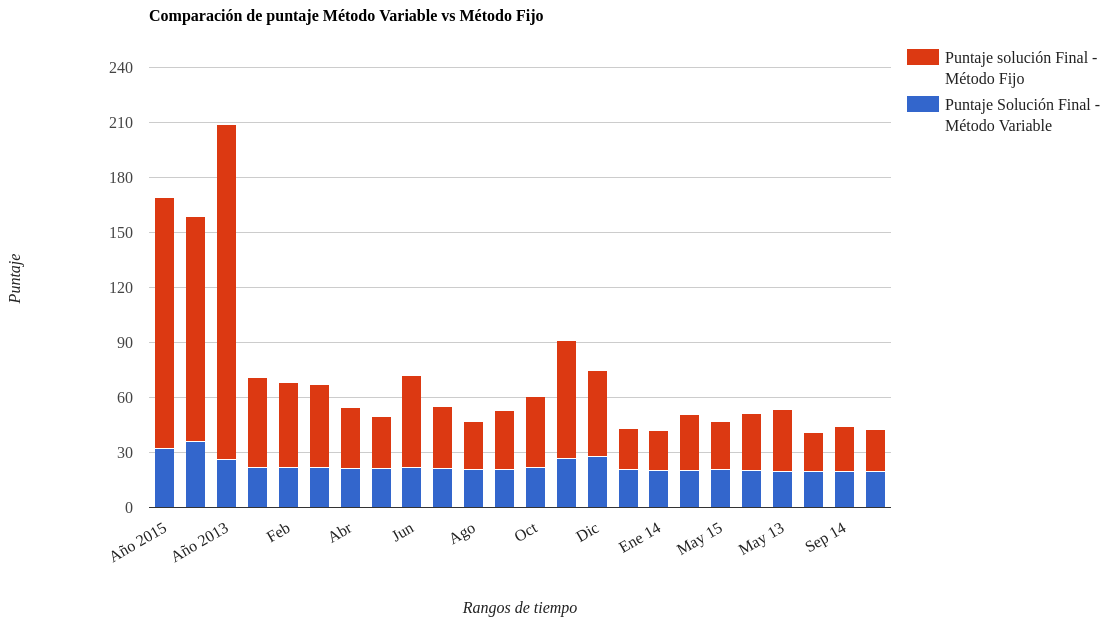
\includegraphics[width=\textwidth]{figures/comp_v1_v2_puntaje.png}
    \end{center}    
    \caption{Comparación de variaciones en el PSO.\\ Fuente: Elaboración propia.}
    \label{fig:comparison_pso_1}
\end{figure}

\begin{figure}[ht!]
    \begin{center}
        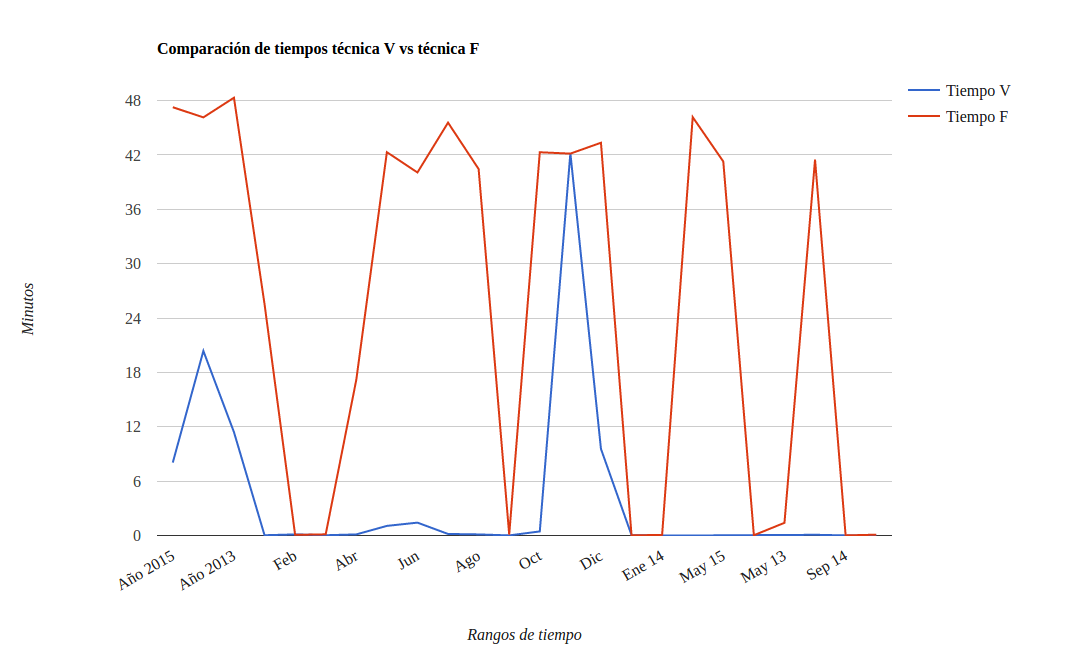
\includegraphics[width=\textwidth]{figures/comp_v1_v2_tiempo.png}
    \end{center}    
    \caption{Comparación de variaciones en el PSO.\\ Fuente: Elaboración propia.}
    \label{fig:comparison_pso_2}
\end{figure}
Los gráficos en \ref{fig:comparison_pso_1} y  \ref{fig:comparison_pso_2} muestran la comparación de los rendimientos de los algoritmos con parámetros fijos y variables para el PSO según la propuesta realizada \ref{eq:VariationParameters_new}. Es claro que en la maýoría de los experimentos, la propuesta realizada tiene mejor rendimiento y en el peor de los casos se comporta igual o levemente peor que la forma tradicional de parámetros fijos utilizada en el trabajo de Heckenbergerova et al. \cite{Heckenbergerova15}.

\pagebreak
\subsection{Aplicaciones}
%%ENERGIA ELECTRICA!!


\pagebreak
\subsection{Conclusiones}
Para obtener información para alguna investigación relacionada a la velocidad del viento en una zona es necesario obtener un modelo que permita explicar las mediciones que se obtienen. Para ello, la distribución de Weibull es una de las funciones más utilizadas para el ajuste de los datos.
Distintos casos de estudio alrededor del mundo demuestran la utilidad de la distribución, utilizando diversos métodos para encontrar los parámetros de ajuste.
En este punto, la meta-heurística \emph{Particle Swarm Optimization} ha demostrado ser una alternativa eficiente para este problema, otorgando soluciones 
de alta calidad.\\
En este trabajo se presentó un caso de estudio para los datos del viento en Valparaíso, en donde los resultados muestran que la distribución de Weibull
se ajusta a la distribución de datos de promedios diarios de velocidad del viento. Esto quiere decir, que si estimamos la velocidad más probable, por ejemplo, 
esta se referirá al promedio más probable que se dé cierto día. Teniendo esto en cuenta, es posible obtener modelos para distintos intervalos de tiempo,
teniendo en cuenta que es posible modificar la calidad del modelos obtenido, mediante el ajuste de los parámetros de la distribución de Weibull.


%%% IMPORTANTE DESTACAR QUE INDEPENDIENTE DE LA NATURALEZA DE LOS DATOS ESTA COSA SE AJUSTA .